\documentclass[12pt]{article}
\usepackage[final]{graphicx}

\usepackage{float}
%\usepackage[caption = false]{subfig}

\usepackage[lofdepth,lotdepth]{subfig}

\title{Lane Detecion Project}
\author{Mingrui Wu}
\date{}

\begin{document}

\maketitle


\section{Camera Calibration}
Camera clibaration is done by following the materials taught in the class. Twenty chess board images are provided in the camera\_cal folder. 
\begin{enumerate}
	\item For each image, find the inner corners by $cv2.findChessboardCorners$. For this function the number of corners in x and y direstions are 9 and 6 respectively.
	\item Append the corners found in the previous step to an array $imgpoints$, at the same time append pre-calculated mesh grid points to another array $objp$
	\item Having scanned all the twenty images, apply $cv2.calibrateCamera$ to calcuate the calibration paramters
	\item For each of the twenty images, apply $cv2.undistort$ to correction the distortion, where the calibration parameters needed by this function are computed in the last step.
\end{enumerate}
	 
An example of camera calibration is given in image \ref{camera_calib}. The two images in the left column are the inpute images, while the two in the right column are the images after distortion correction.

\begin{figure}[h]
\centering
\subfloat[input image]{
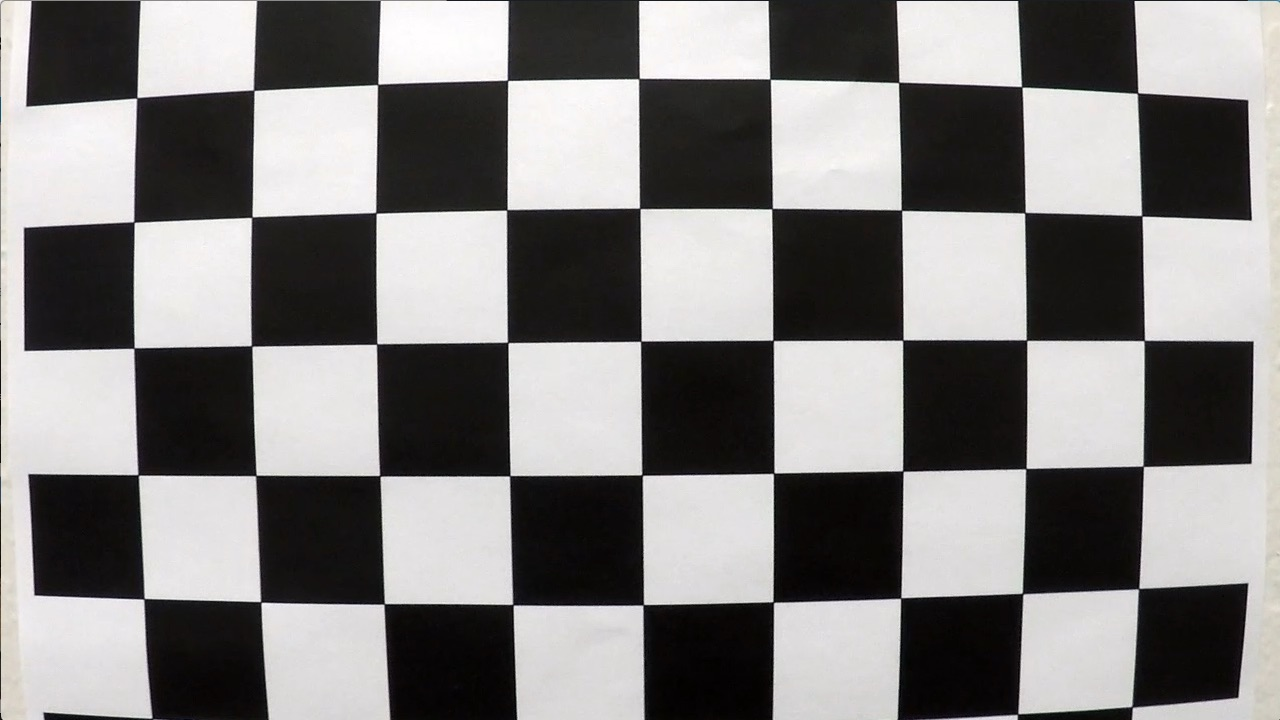
\includegraphics[width=0.4\textwidth]{calibration1.jpg}
\label{fig:input}}
\qquad
\subfloat[undistorted image]{
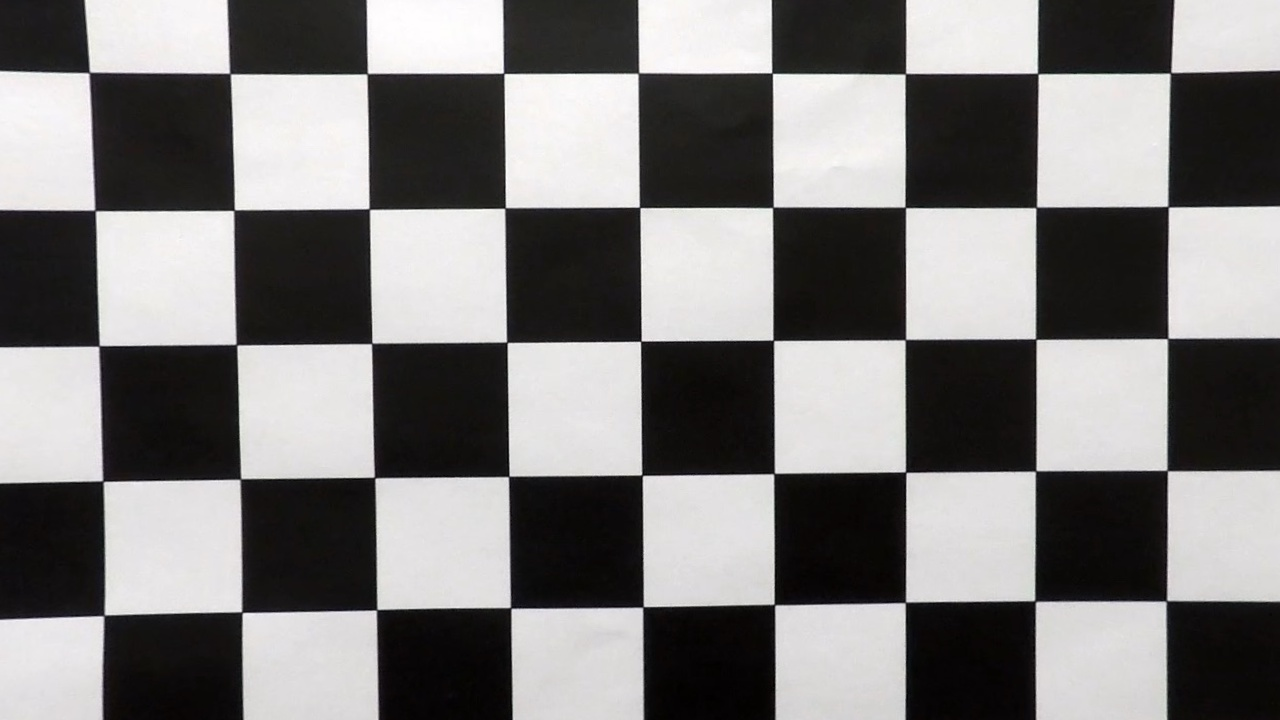
\includegraphics[width=0.4\textwidth]{undist_calibration1.jpg}
\label{fig:camera_calib}}
\qquad
\subfloat[input image]{
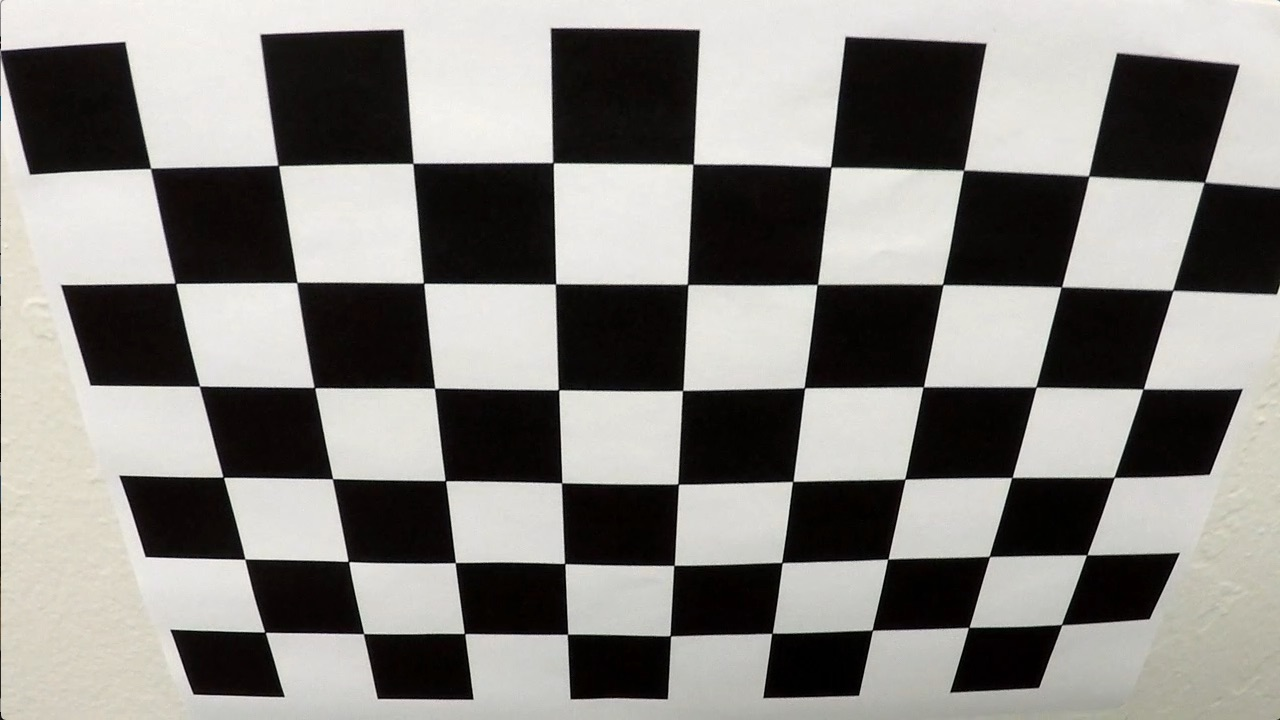
\includegraphics[width=0.4\textwidth]{calibration2.jpg}
\label{fig:input}}
\qquad
\subfloat[undistored image]{
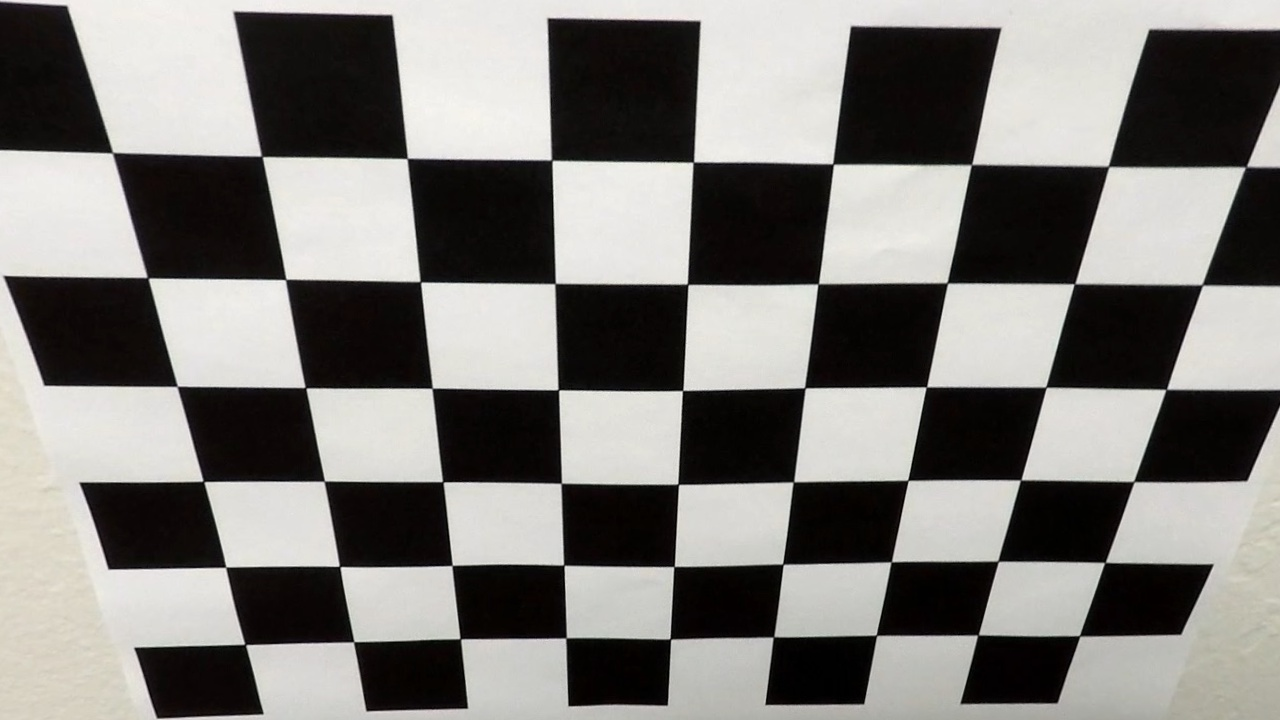
\includegraphics[width=0.4\textwidth]{undist_calibration2.jpg}
\label{fig:camera_calib}}
\caption{Camera calibration}
\end{figure}

The undisorted images for all the twenty images provided in the  camera\_cal folder can be found in  camera\_cal/calib\_result folder.
  
    
\section{Pipline}
In my code, py/lane\_detector.py is the class for performing lane detection. Within this class, the member function lane\_detect describes the whole pipeline.

Take the input image Fig \ref{fig:input} as an example, the whole piple line consists of the following steps:

\begin{enumerate}
	\item \textbf{Distortion correction.} Using the pre-calculated camera calibration parameters mentioned in the last section, the first step is to apply $cv2.undistort$ to the input image to get the undistorted image. The undistorted result for \ref{fig:input} is given in \ref{fig:undistort}

	\item  \textbf{Binary thresholding} This is 

		\begin{enumerate}
			\item \textbf{Color mask.} Similarly to what was taught in the class, A color mask is built to mark the interest areas based on the colors. First the yellow areas are detected based on a given HSV range. Then the white areas are detected based on both RGB and HSV ranges. And a bit OR is performed to produce the combined color mask. The yellow mask, white mask and the color mask are shown in Fig. \ref{fig:yellow_mask}, Fig. \ref{fig:white_mask} and Fig. \ref{fig:color_mask} respectively. Note that the white mask this example is not accurate, since I use a relaxed range parameters for color detection. This is to retain engouh edge pixles later in all kinds of light/color conditions.

			\item  \textbf{Interest region mask.} A trapzoid shape region at the bottom of the image is marked as the interest region mask. An interest region mask is shown in Fig \ref{fig:region_mask}.
		\end{enumerate}

	\item \textbf{Edge image.} As suggested in the class, a Gaussian smoothing is performed, followed by the Canny edge detection operator. This step results in a edge image, which gives the pixels which have strong intensity gradients. An edge image is shown in Fig \ref{fig:edge}.
	
	\item \textbf{Masked edge image.} The edge image and the candiate region mask are combined by performing the bit AND operation, which produces a masked edge image. A masked edge image is shown in Fig \ref{fig:masked_edge}.
	
	\item \textbf{Lane line segments.} Following the class, Hough transform is peformed upon the masked edge image obtained in the last step. This can detect the lane segments, which is requested in the first task of this project. The detected lane line segments are shown in Fig \ref{fig:line_segment}. The input image combine with the line segments is shown in Fig \ref{fig:combined_line_segment}.
	
	\item \textbf{Full extent of lane lines.} To accomplish the second task of this project, we need to combine the line segments into two full extent lane lines, the left line and right line. The details of this step will be explained in the next section. The constructed full lines are shown in Fig \ref{fig:full_line}. The input image combined with detected full extent of lane lines is shown in Fig \ref{fig:combined_full_line}.
\end{enumerate}

\begin{figure}[h]
\centering
\subfloat[input image]{
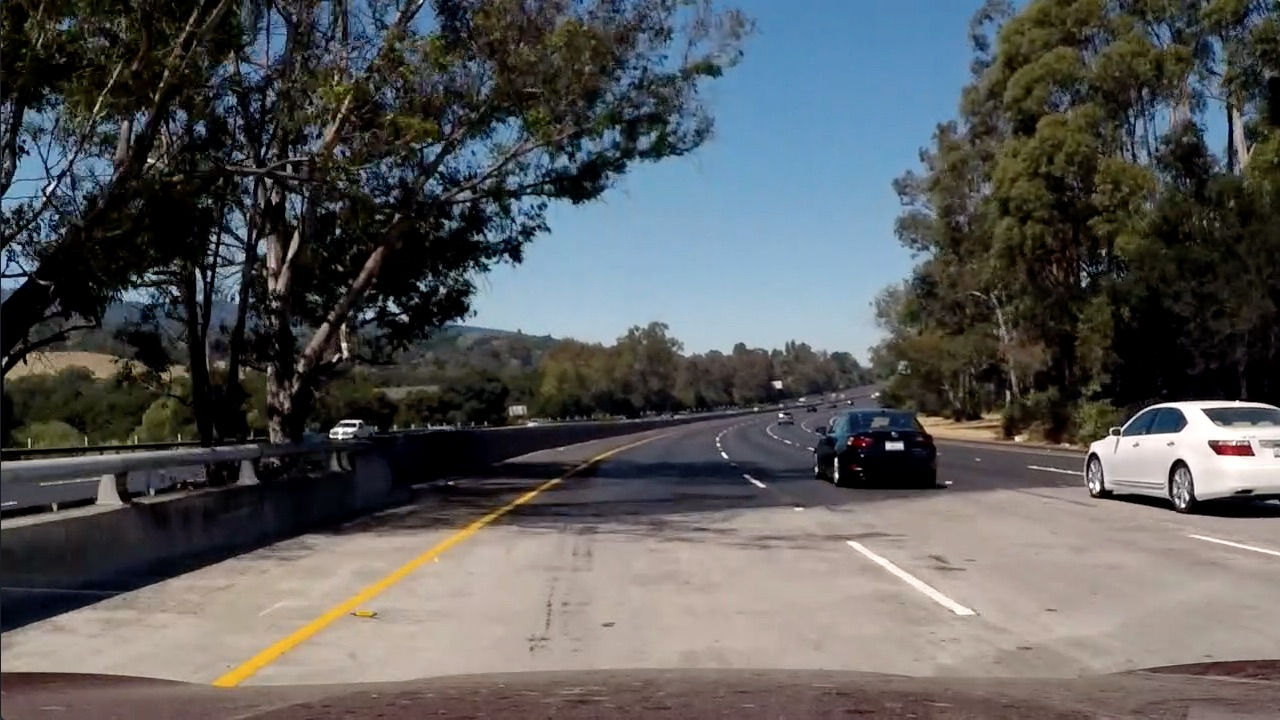
\includegraphics[width=0.4\textwidth]{test5.jpg}
\label{fig:input}}
\qquad
\subfloat[undistorted image]{
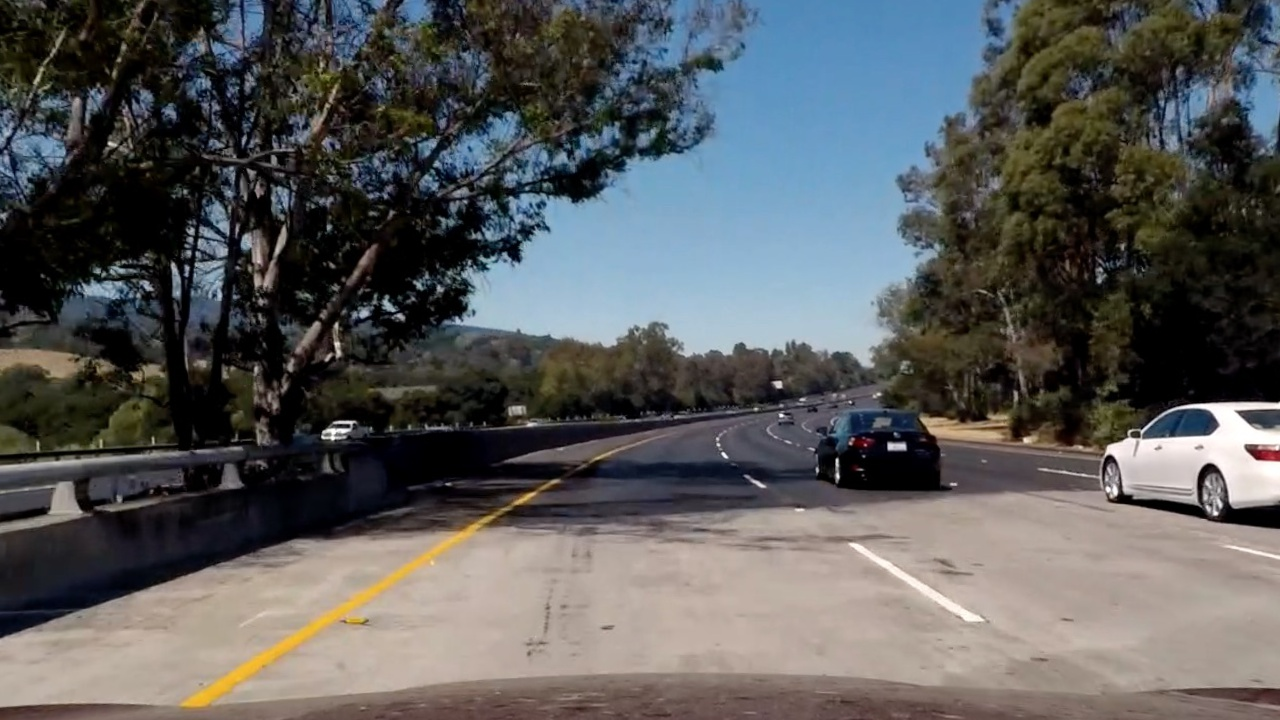
\includegraphics[width=0.4\textwidth]{undist_test5.jpg}
\label{fig:undistort}}
\caption{Lane detection pipeline}
\end{figure}

\section{Full extent of lane lines}
This section explains the last step of the pipeline. This in turn contains two steps. 

\subsection{Grouping line segments into left and right}
In the second last step, a set of line segments are obtained by Hough transform. These line segments are grouped into left and right lines respectively, based on the slopes. The line segments with negative slopes are put into the left group, while the line segments with the positive slopes are put into the right group. In implementation, to filter out some noisy line segments, only the line segments whose slopes are within the given slope ranges are considered, while the other line segments are ignored. The slope ranges are parameters need to be tuned. And there is one slope range for the left group and the right group respectively.

\subsection{Forming the full lane lines}
Having obtained left and right groups of line segments, we need to form one line from each group. Two approaches have been tried.

\subsubsection{Avearing the line segments in one group}
For each group of line segments, this approach simply builds the full extent line by averaging the slopes and interceptions of the line segments in the group. This approach works in most cases. However it is not robust since it can be eaily disturbed by some nosisy slope or interception values. For example, if some line segments' slopse or/and interceptions are far away from the ground true, even those short segments are located within the true lane lines, averaging can still result in the slopes/interceptions that are quite different from those of the true land lines. This problem can be alleviated by fine tuning the parameters, but I am trying to find some better approaches.

\subsubsection{Robust line fitting with RANSAC}
The above approach is not robust since averaging slopes and interceptions can be easily disturbed by outlier segments even when those outliers are located within the true lane lines.

Based on the above observation, instead of computing the slopes and interceptions by averaing, I turn to fit one line robustly for each group, left and right respectively. So for each group, we just need to fine one line that are close to the end points of the line segments in the group. This can overcome the problem in the averaging approach: as long as the line segments are within the true lane lines, this can produce the ideal result even when the slopes/interceptions of those segments are quite different from those of the true lane lines. For the nosity line segments that are located far away from the lane lines, RANSAC algorithm can ignore them automatically.

This approach works very well on the test videos. It gives good estimation in almost all the frames.



\section{Problems and possible improvements}
The above pipeline works pretty well on the given test images and test videos. However, it breaks on some parts of the challenging video, challenge.mp4. The reason is that in the chanllenge.mp4, there are some strong edges: the car itself and the color change of the road. A failure example is shown in Fig \ref{fig:failure}. 

I tried to fine tunning the parameters for color detection, since the pixles around those edges are neither white nor yellow. However, mannully tunning the parameters can be suffering. It may improve the results on some particular frames while break the results on some other frames. Probably a more principaled way like building a trained model which considers both color and edge information can get a better result.


\end{document}
